\documentclass[12pt,a4paper]{article}
\usepackage[utf8]{inputenc}
\usepackage[spanish]{babel}
\usepackage{amsmath}
\usepackage{amsfonts}
\usepackage{amssymb}
\usepackage{makeidx}
\usepackage{graphicx}
\usepackage{lmodern}
\usepackage{kpfonts}
\usepackage{fourier}
\usepackage[left=2cm,right=2cm,top=2cm,bottom=2cm]{geometry}
\author{Joan Moran - Carolina González - Ronaldo Larrosa}
\title{Proyecto}
\begin{document}
\maketitle Proyecto Segundo Parcial Proceso de Software 
\newpage
\tableofcontents
\newpage

\section{Normas ISO}

ISO (Organización Internacional de Normalización) es una federación mundial de organismos nacionales de normalización (organismos miembros de ISO). El trabajo de preparación de las normas internacionales normalmente se realiza a través de los comités técnicos de ISO. Cada organismo miembro interesado en una materia para la cual se haya establecido un comité técnico, tiene el derecho de estar representado en dicho comité. Las organizaciones internacionales, públicas y privadas, en coordinación con ISO, también participan en el trabajo. ISO colabora estrechamente con la Comisión Electrotécnica Internacional (IEC) en todas las materias de normalización electrotécnica.\\
\subsection{Norma ISO 9001}


La Norma ISO 9001 especifica los requisitos para un sistema de gestión de la calidad que pueden utilizarse para su aplicación interna por las organizaciones, para certificación o con fines contractuales. Se centra en la eficacia del sistema de gestión de la calidad para satisfacer los requisitos del cliente.\\

\section{Caso de Estudio}
Un museo vivo para la pantalla de inicio de tu Android.\\
Muzei es un fondo de pantalla en vivo que actualiza suavemente su pantalla de inicio cada día con famosas obras de arte. También retrocede hacia el fondo, difumina y atenúa las ilustraciones para mantener sus íconos y widgets en el centro de atención. Simplemente toque dos veces el fondo de pantalla o abra la aplicación Muzei para disfrutar y explorar la obra de arte en todo su esplendor.\\

Alternativamente, puede elegir sus fotos favoritas de su propia galería u otras aplicaciones para usar en su pantalla de inicio. Para mantener su fondo de pantalla fresco, Muzei rotará a través de sus fotos favoritas después de un determinado tiempo.\\

\begin{Imagen}
\centering
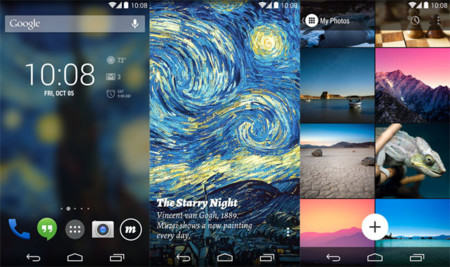
\includegraphics[scale=0.9]{Imagen.jpg}
\caption{Muzei}
\end{Imagen}

\section{Requerimientos}
a)	Es una aplicación que actualizará el fondo de pantalla del móvil.\\
b)	Disminuir la intensidad para mantener la visibilidad de los iconos.\\
c)	Requiere Android 4.2 o superior\\

\section{Contexto del Proyecto}

Muzei es un fondo de pantalla en vivo que refresca suavemente la pantalla de inicio cada día con obras de arte famosas. También retrocede en el fondo, difuminando y atenuando las ilustraciones para mantener sus íconos y widgets en el centro de atención. Simplemente toque dos veces el fondo de pantalla o abra la aplicación Muzei para disfrutar y explorar la obra de arte en todo su esplendor.\\

Alternativamente, puede elegir sus fotos favoritas de su propia galería u otras aplicaciones para usar en su pantalla de inicio. Para mantener fresco el fondo de pantalla, Muzei rotará a través de tus fotos favoritas cada pocas horas.\\

Finalmente, Muzei es amigable para los desarrolladores. Todo el código está disponible en http://code.muzei.co y Muzei incluso ofrece una API simple que le permite crear su propia fuente de fondo de pantalla. Para detalles de API, visite http://api.muzei.co.\\

Si utiliza una Fuente heredada de terceros, debe desactivar las Optimizaciones de la batería en esa aplicación para permitir que continúe cargando las ilustraciones. Consulte https://medium.com/muzei/muzei-3-0-and-legacy-sources-8261979e2264 para obtener más detalles.\\


Muzei ahora incluye una carátula para Android Wear, ¡para que puedas ver tu último fondo de pantalla directamente en tu muñeca!\\


Hecho por Roman Nurik e Ian Lake, junto con las contribuciones de muchos en la comunidad de Android. Muzei es una transliteración de la palabra rusa музей, que significa "museo".\\

Las obras de arte destacadas en Muzei están a diario a cargo de nuestro reducido personal y son posibles gracias a WikiArt.org y sus colaboradores.\\

\section{Link del Repositorio}
El repositorio del presente proyecto de encuentra en la siguiente dirección: \\
https://github.com/joan2211/ProyectoSegundoParcial


\end{document}